\cotefile{156-9}
\scanpage{90}
\mspage{86}
% archive sheet number: 89

et \unsure{on} trouve la $=$ interprétation pour le $2^{\mathrm e}$ \unsure{mbr|membre} de $\unsure{\alpha|\infty}$.

Soient maintenant $(E,\mid\circ\mid_E)$, $(E',\mid\circ\mid_{E'})$ deux \unsure{disjoncteurs}, et considérons deux correspondances
\[
\begin{aligned}
\alpha &: E \unsure{\text{---}|\longrightarrow} \unsure{\mathscr{P}|\mathcal{P}}(E') \quad,\quad \bar\alpha : \mathscr{P}(E)\unsure{\text{---}|\longrightarrow}\mathscr{P}(E')\\
\beta &: E'\unsure{\text{---}|\longrightarrow}\mathscr{P}(E) \quad,\quad \bar\beta : \mathscr{P}(E')\unsure{\text{---}|\longrightarrow}\mathscr{P}(E)
\end{aligned}
\]

\deleted{\uline{\unsure{Lemme 1}}}\inserted{Prop. 3} Conditions équivalentes
% Long vertical grouping stroke beside conditions (i)--(iii).
\figure{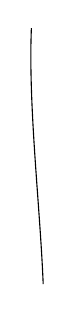
\begin{tikzpicture}[x=0.5cm,y=0.5cm]
\draw (0,6.5) .. controls (-0.08,4.5) and (0.22,2) .. (0.3,0);
\end{tikzpicture}}

(i) $\forall x\in E,\ x'\in E'$, on a
\[
x\mid\circ\mid\beta(x')\ \Longleftrightarrow\ \alpha(x)\mid\circ\mid x'
\]

(ii) $\forall A\subset E,\ A'\subset E'$, on a
\[
A\mid\circ\mid\bar\beta(A')\ \Longleftrightarrow\ \bar\alpha(A)\mid\circ\mid A'
\]

(iii) Posant, pour $\unsure{\mathscr{S}|\mathfrak{S}|\mathbb{S}}\in\deleted{\unsure{\mathscr{P}(E)}}\Sigma_E,\ \mathscr{S}'\in\Sigma_{E'}$
\[
\begin{aligned}
\alpha_{\unsure{*|\ell}}(\mathscr{S})&=\operatorname{supp}^{\circ}_{E'}(\bar\alpha(\mathscr{S}))\\
\beta_*(\mathscr{S}')&=\operatorname{supp}^{\circ}_E(\bar\beta(\mathscr{S}'))
\end{aligned}
\]
\unsure{a)} On a \deleted{\unsure{pour}} l'équivalence
\[
\deleted{\unsure{\alpha_*(A)}}\mathscr{S}\mid\circ\mid\beta_*(\mathscr{S}')\ \Longleftrightarrow\ \alpha_*(\mathscr{S})\mid\circ\mid\mathscr{S}'
\]
\inserted{b) \deleted{plus} les relations, pour $A\in\mathscr{P}(E),\ A'\in\mathscr{P}(E')$ :}
\[
\begin{aligned}
\inserted{\alpha_*(\operatorname{supp}^{\circ}_E(A))=\operatorname{supp}^{\circ}_{E'}(\bar\alpha(\unsure{A'|A}))}\\
\inserted{\beta_*(\operatorname{supp}^{\circ}_{E'}(A'))=\operatorname{supp}^{\circ}_E(\bar\beta(\unsure{B|A'})))}
\end{aligned}
\]
\deleted{De plus,}\quad\deleted{\unsure{Démonstration.}}

% margin note written sideways, slanted upwards to the right
\margin{\uline{Définition} On dit \unsure{donc|alors} \unsure{que} $\alpha$ et $\beta$ sont \inserted{\uuline{\unsure{pré}}}\unsure{transposés} l'un de l'autre.}

% The following block is crossed through by long diagonal strokes.
\deleted{\uline{\unsure{(iv)}} Ces conditions ne dépendent que des applications $\alpha_*,\beta_*$}
% Curved stroke at the left of the cancelled lower block.
\figure{\begin{tikzpicture}[x=0.5cm,y=0.5cm]
\draw (0,2.2) .. controls (-0.18,1.4) and (-0.18,0.7) .. (0.18,0);
\end{tikzpicture}}
\[
\deleted{\unsure{\alpha_*:}}
\]
\diagram{\begin{tikzcd}[ampersand replacement=\&]
\deleted{\Sigma_E}\arrow[r,shift left=0.6ex,"\deleted{\alpha_*}"] \& \deleted{\Sigma_{E'}}\arrow[l,shift left=0.6ex,"\deleted{\beta_*}"]
\end{tikzcd}}
\deleted{définies \unsure{$\beta$} par $\alpha$ et $\beta$, et en particulier ne changent pas quand on remplace $\alpha$ et $\beta$ par $\alpha',\beta'$ \unsure{définis} par}
\[
\deleted{\unsure{\alpha}\quad\alpha(x)=\operatorname{supp}^{\circ}_E\alpha(x)}
\]
% slanted
\margin{\uline{\unsure{Donc}}}
